\documentclass[10pt]{article}\usepackage[]{graphicx}\usepackage[]{color}
%% maxwidth is the original width if it is less than linewidth
%% otherwise use linewidth (to make sure the graphics do not exceed the margin)
\makeatletter
\def\maxwidth{ %
  \ifdim\Gin@nat@width>\linewidth
    \linewidth
  \else
    \Gin@nat@width
  \fi
}
\makeatother

\usepackage{Sweavel}


\usepackage{hyperref}
\usepackage{url}
\usepackage[a4paper]{geometry}
\usepackage{a4wide}
\usepackage{float}
\usepackage[english]{babel}
\usepackage[utf8]{inputenc}
\usepackage{csquotes}
\usepackage{amsmath}
\usepackage{amssymb}
\usepackage{xspace}
\usepackage[numbers]{natbib}
\bibliographystyle{unsrtnat}
\usepackage{subcaption}
\usepackage[font={small}]{caption}
\usepackage{booktabs}
\usepackage{listings}
\usepackage{cleveref}
\usepackage{lipsum}
\usepackage{graphicx}
\usepackage{epstopdf}
\graphicspath{{../figures/}}
\epstopdfsetup{outdir=./}
\newcommand{\approxtext}[1]{\ensuremath{\stackrel{\text{#1}}{=}}}
\newcommand{\matr}[1]{\mathbf{#1}}
\newcommand{\partt}[2]{\ensuremath{\dfrac{\partial {#1}}{\partial {#2}}}}
\renewcommand{\d}[1]{\ensuremath{\operatorname{d}\!{#1}}} % non-italized differentials
\newcommand{\h}[0]{\ensuremath{\hbar}} % hbar
\def\changemargin#1#2{\list{}{\rightmargin#2\leftmargin#1}\item[]}
\let\endchangemargin=\endlist 
\usepackage{amsthm}
\theoremstyle{plain}
\renewcommand{\theequation}{\thesection.\arabic{equation}}
\def\changemargin#1#2{\list{}{\rightmargin#2\leftmargin#1}\item[]}
\let\endchangemargin=\endlist    
\usepackage{xcolor}
\definecolor{Red}{rgb}{0.7,0,0}
\definecolor{Blue}{rgb}{0,0,0.8}
\usepackage{verbatim}
\def\changemargin#1#2{\list{}{\rightmargin#2\leftmargin#1}\item[]}
\let\endchangemargin=\endlist
\addtolength{\oddsidemargin}{-.35in}
\addtolength{\evensidemargin}{-.35in}
\addtolength{\textwidth}{.7in}
\usepackage{multicol}

% Stephen's stuff
\newcommand{\R}{\texttt{R}}
\newcommand{\Rfunction}[1]{{\texttt{#1}}}
\newcommand{\Robject}[1]{{\texttt{#1}}}
\newcommand{\Rpackage}[1]{{\mbox{\normalfont\textsf{#1}}}}
\usepackage{xcolor}
\definecolor{Red}{rgb}{0.7,0,0}
\definecolor{Blue}{rgb}{0,0,0.8}
\hypersetup{%
pdfusetitle,
bookmarks = {true},
bookmarksnumbered = {true},
bookmarksopen = {true},
bookmarksopenlevel = 2,
unicode = {true},
breaklinks = {false},
hyperindex = {true},
colorlinks = {true},
linktocpage = {true},
plainpages = {false},
linkcolor = {Blue},
citecolor = {Blue},
urlcolor = {Red},
pdfstartview = {Fit},
pdfpagemode = {UseOutlines},
pdfview = {XYZ null null null}
}
%% Listings
\lstset{ 
language=R,                     % the language of the code
basicstyle=\footnotesize,       % the size of the fonts that are used for the code
numbers=left,                   % where to put the line-numbers
numberstyle=\tiny\color{gray},  % the style that is used for the line-numbers
stepnumber=1,                   % the step between two line-numbers. If it's 1, each line will be numbered
numbersep=5pt,                  % how far the line-numbers are from the code
backgroundcolor=\color{white},  % choose the background color. You must add \usepackage{color}
showspaces=false,               % show spaces adding particular underscores
showstringspaces=false,         % underline spaces within strings
showtabs=false,                 % show tabs within strings adding particular underscores
rulecolor=\color{black},        % if not set, the frame-color may be changed on line-breaks within not-black text (e.g. commens (green here))
tabsize=2,                      % sets default tabsize to 2 spaces
captionpos=b,                   % sets the caption-position to bottom
breaklines=true,                % sets automatic line breaking
breakatwhitespace=false,        % sets if automatic breaks should only happen at whitespace
title=\lstname,                 % show the filename of files included with \lstinputlisting;
% also try caption instead of title
keywordstyle=\color{Blue},      % keyword style
commentstyle=\color{orange},    % comment style
stringstyle=\color{Red},        % string literal style
escapeinside={\%*}{*)},         % if you want to add a comment within your code
morekeywords={*,...}            % if you want to add more keywords to the set
} 

\epstopdfDeclareGraphicsRule{.tga}{png}{.png}{%
  convert #1 \OutputFile
}
\AppendGraphicsExtensions{.tga}

%%% Document specific
\newcommand{\course}{Structural Biology}
\newcommand{\ass}{1}
\newcommand{\term}{Lent term 2017}
%\bibliography{pga1}

%%% Title page
\title{
  \bf \course: Assignment \ass \\[1em]
  \small{University of Cambridge}
}

\author{Henrik Åhl}
\date{\today}
\renewcommand{\textfraction}{0.05}
\renewcommand{\topfraction}{0.8}
\renewcommand{\bottomfraction}{0.8}
\renewcommand{\floatpagefraction}{0.75}

%%% Actual document
\begin{document}
\date{\today}
\maketitle
\setcounter{page}{1}


% \date{\today}
\maketitle
\begin{abstract}
	{\bf 
		%\begin{changemargin}{-.8cm}{-.8cm}
		This is an abstract abstract.
	}
\end{abstract}

\begin{multicols*}{2}
	\section*{Preface}
	This is an assignment report in connection to the \textit{\course}
	module in the Computational Biology course at the University of Cambridge,
	\term. All related code is as of \date{\today} available through a
	Github repository by contacting \href{mailto:hpa22@cam.ac.uk}{hpa22@cam.ac.uk}.
	
	\section*{Exercises}
	\subsection*{1}
	How would you describe its structure? 
	
	The protein in essence consists of a toroidal structure made up by anti-parallel
	beta-sheets. These are separated into two sub-structures of 6 and 3 beta-strands
	each. Together, the structure forms a seemingly twisted, tubular form, making it
	seem like the top conformation is made out to capture incoming molecules of some
	sort. Even though this might be because of resolution issues, water molecules do
	not appear to be present within the structure, or at least not frequent. Maybe
	electrostatically repelled? 
	
	% \begin{figure}[H]
	%   \centering
	%   \includegraphics{../figures/prot1_topview}
	%   \caption{topview}
	%   \label{fig:topview}
	% \end{figure}
	% 
	% \begin{figure}[H]
	%   \centering
	%   \includegraphics{../figures/prot1_aligned}
	%   \caption{aligned}
	%   \label{fig:aligned}
	% \end{figure}
	
	In aligning the structures, we can clearly see how the “entrance” to the
	capturing cavity is inaccessible in the starting structure (i.e.\ during X-ray
	crystallography). Aside of the general opening in the structure, the red
	(opening) appears to have a slightly bigger cavity. 
	
\begin{Schunk}
\begin{figure}[H]

{\centering 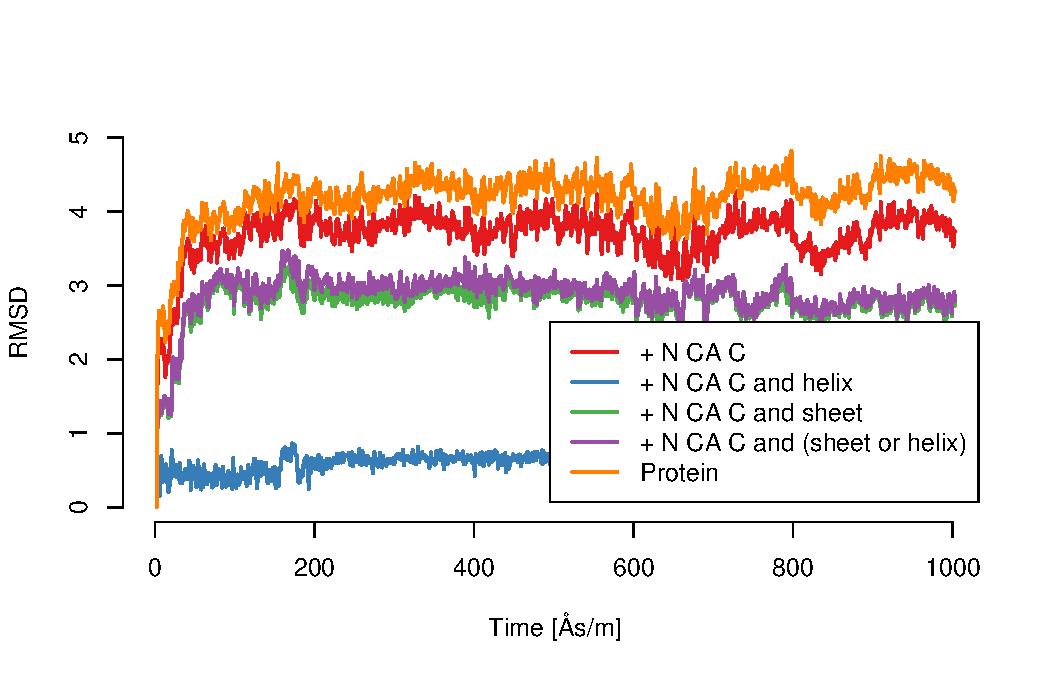
\includegraphics[width=\maxwidth]{figure/twocolumn-trajs-1} 

}

\caption[Things]{Things}\label{fig:trajs}
\end{figure}
\end{Schunk}
\end{multicols*}

\begin{figure}[H]
	\centering
	\includegraphics[trim={2cm 1.6cm 0 0}, clip, width = \textwidth]{../figures/timeline}
	\caption{timeline}
	\label{fig:timeline}
\end{figure}
\begin{multicols*}{2}
	
	Formation of new (pink) domains. Amino acid involved in forming helix very variable. Most domains fairly stable overall, but most also alternate at some point. 
	
	INCLUDE PINK DOMAIN THINGY
	\begin{figure}[H]
		\centering
		\includegraphics[trim={9cm 8cm 9cm 6cm}, clip, width = .3\textwidth]{../figures/domainchange_snapshot}
		\caption{domainchange}
		\label{fig:domchange}
	\end{figure}
	
	ARG90-XXX120 are the end of one beta-sheet (arrow) and the bottom of another. SER120 is the 3-one (head), whereas ARG90 is the 6-one (bottom). 
	
	SER27-PRO50 are on the other side of the 3-domain, and  
	
	% PLOT FIGURE OF THE THREE REGIONS HERE. 
	
	
	\subsection{9}
	\begin{figure}[H]
		\centering
		\includegraphics[trim={2cm 2.5cm 5cm 4.5cm}, clip, width = .45\textwidth]{../figures/charged}
		\caption{charged}
		\label{fig:charged}
	\end{figure}
	
	Charged guys are far away from the core structure. 
	
	The flexible structures of the protein also tends to consist of smaller amino acids (the spaghetti-like things) (plotting "small" residues)
	
	No ions in complex.
	
	Almost no overlap between polar and hydrophobic amino acids.
	
	
	\subsection{10}
	Non-functional form: Water molecules in cavity.
	Functional form: No water molecules in cavity.
	
	\subsection{11}
	The molecule stays pretty much the same, with the ring inside of the cavity. In the end, it comes together with the other other side of the cavity. It has also functionally "bent over", i.e.\ so that it hangs "inwards" from the other side of the cavity. A 180+ degree rotation around it's axis.  
	
	
	
	
	\bibliography{references}
\end{multicols*}
\end{document}
